\chapter{Methodology}
\label{sec:training}

\section{Data Generation}

\begin{figure}[htbp]
	\centering
	\includegraphics[width=\textwidth]{fig/datagen_notation}
	\caption{Overview of the data generation process.}
	\label{fig:training:datagen_notation}
\end{figure}

In order to to investigate the research questions a data generation pipeline is implemented using OpenGL, UnrealEngine and AirSim. An overview can be seen in \Cref{fig:training:datagen_notation}. In the first step a scene is created in which the objects of interest as well as the camera are placed. In 3D space position and orientation (pose) of each object are determined by translation $\textbf{t}$ and rotation $\textbf{r}$. The coordinate system is \ac{NED}.

A view projection yields an image through the lens of the camera. The coordinates of each point in 3D space are projected on the 2D image plane. A final post processing step can simulate further effects like lens distortion and sensor noise. This step is implemented using OpenCV and Python.

All source code is made publicly available at \url{https://github.com/phildue/datagen.git}.

Within the pipeline environments for training and testing are created. A black environment serves as base to replace the background with existing images. Furthermore, three indoor base environments are created that fully simulate illumination and background. An overview can be seen in \Cref{fig:environments}. Within the environment light conditions, background textures, object locations can be changed manually. The environments are described in the following:

\begin{enumerate}
	\item \textit{Dark:} The environment is a room without windows, only containing artificial light sources. 
	\item \textit{Daylight:} The environment is a room with windows along all walls that allow daylight to illuminate the room. The windows can lead to strong variations in the contrast between different parts of the object.
	\item \textit{IROS:} The environment resembles the room of the \ac{IROS} Autonomous Drone Race 2018. The light sources stem from a window front at one side of the room, as well as artificial light sources at the ceiling. Depending on the view point, the object might appear against bright or dark background.
\end{enumerate}

\begin{figure}[hbtp]
	\centering
	\begin{minipage}{0.3\textwidth}
		\includegraphics[width=\textwidth]{fig/basement_perspective}
	\end{minipage}
	\begin{minipage}{0.3\textwidth}
		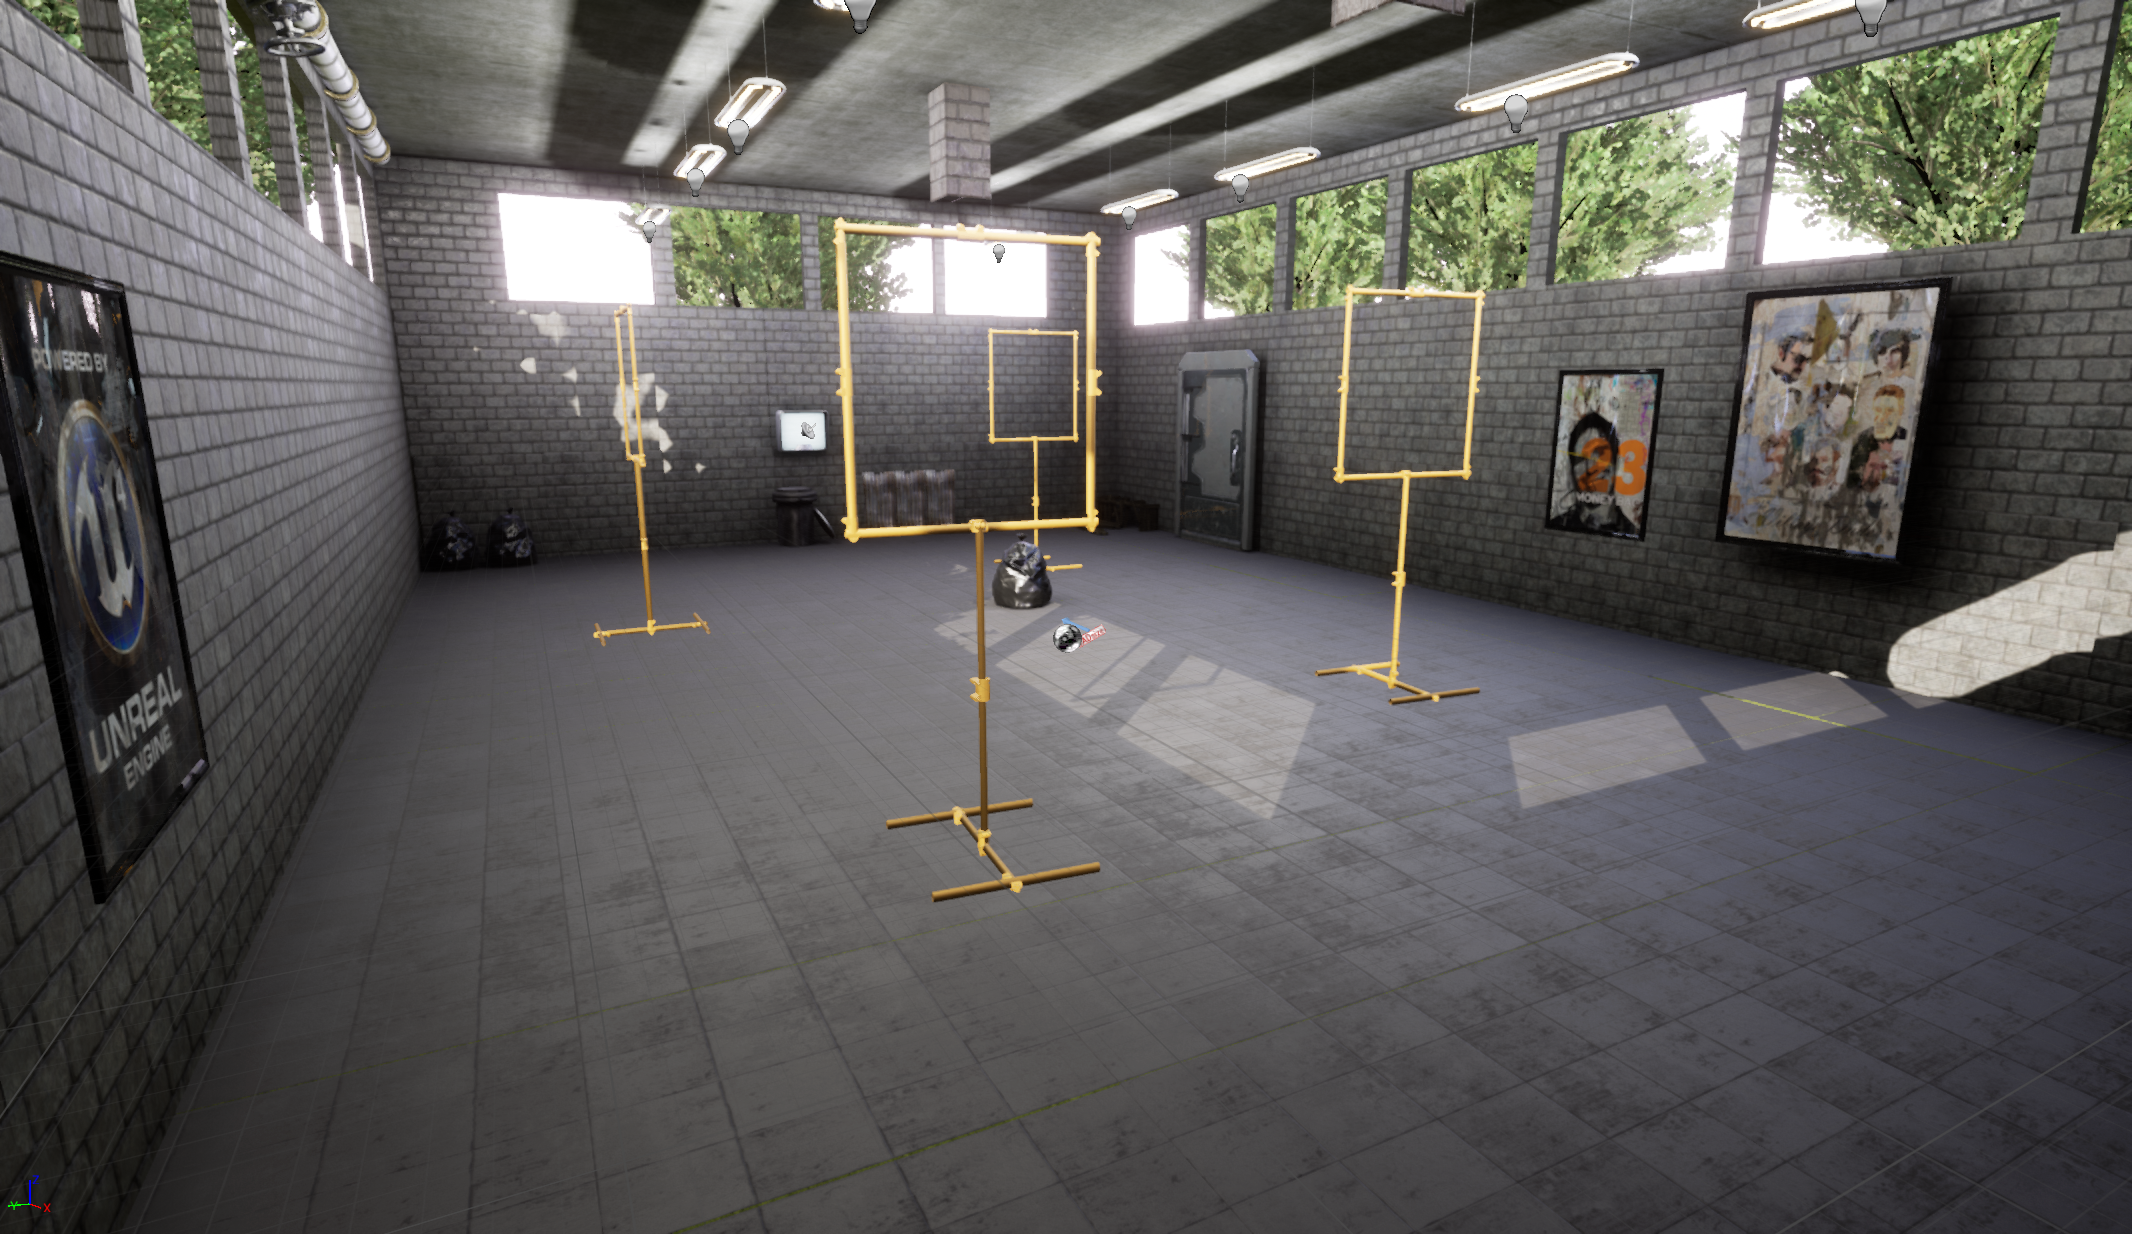
\includegraphics[width=\textwidth]{fig/daylight_perspective}
	\end{minipage}
	\begin{minipage}{0.3\textwidth}
		\includegraphics[width=\textwidth]{fig/iros_perspective}
	\end{minipage}
	\caption{\textit{IROS2018} Environment.}
	\label{fig:environments}
\end{figure}

AirSim provides the simulation of dynamics as well as controllers for \acp{MAV}. In order to evaluate the generated models a test set is created by simulating a flight of a \ac{MAV} through a race court. Thereby the race court resembles the course of the Autonomous Drone Race at the IROS 2018 conference. The generated test set contains TODO samples with TODO objects in total.

It should be noted that when generating data with the described methods it is likely that samples appear in which only a corner of the object is visible or the view angle is in such a way that the object appears only as a thin line. In initial experiments these corner cases led to unstable training. Hence, some minimum requirements for the labels are set and samples are removed if these are not met. The criteria are:

\begin{itemize}
	\item Minimum Width/Height: 0.025 Image Width/Height
	\item Minimum Aspect Ratio: 0.3
	\item Maximum Aspect Ratio: 3.0
	\item Minimum Corners Visible: 3
\end{itemize}


\section{Detection Model}
